\documentclass[a4paper,10pt,twoside]{article}

\usepackage{ucs}
\usepackage[utf8]{inputenc}
%\usepackage{babel}
\usepackage{fontenc}
\usepackage[pdftex]{graphicx}

\usepackage[dvips]{hyperref}

\author{Alexander Ekman}
\title{tutorial2a}
\date{09/14/17}

\begin{document}
\maketitle

\begin{center}
\texttt{alexander.ekman95@gmail.com}
\end{center}

\section{Introduction}
\label{sec:intro}

This is introduction. Summary will be given in the Section \ref{sec:sum}

\section{About Linux}
\label{sec:linux}

\begin{figure}[h]
  \begin{center}
 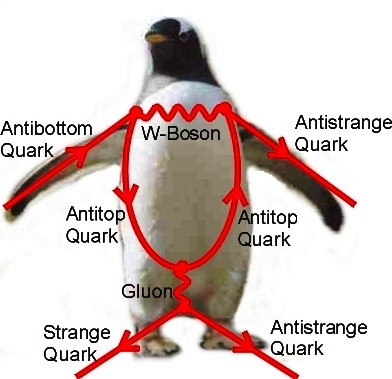
\includegraphics[width=6cm]{penguin.jpg}
 \caption{Penguin represents Linux}
 \label{fig:penguin}
  \end{center}
  
Figure \ref{fig:penguin} shows a \textit{penguin}. For more details, check the Linux Web page~\cite{linux}

\end{figure}

\subsection{Linux Flavours}
\label{sec:flavours}

Table~\ref{tab:flavours} lists some Linux flavours~\footnote{Only one is shown for simplicity}

\begin{table}
 \begin{center}
 
 \label{tab:flavours}
 
  \begin{tabular}{|c|c|c|c|}
    \hline
   \textbf{Distribution}&RedHat&Debian&SuSE\\\hline\hline
   Yakkety Yak		&	&X	&	\\
   \hline
  \end{tabular}
 \caption{Different flavours of Linux}
 \end{center}

\end{table}

\section{About Mathematics}
In-line math in \LaTeX \ is enclosed in \$ symbols. Backslash \textbackslash \
is used ti denote special symbols.

Subscripts and superscripts are always math: $A_x$, $A_{xy}$, $e^x$ and $e^{x^2}$. Using underscore \_ outside math with \textbackslash causes big\_ troubles.

All special symbols are also math: $\alpha$, $\beta$, $\gamma$, $\delta$, $\sinx$, $\hbar$, $\lambda$, $\ldots$. More information can be found in Ref.~\cite{latex}.

Equation~\ref{eq:chi2} shows $chi^2$

\begin{equation}
 \label{eq:chi2}
 \chi^2=\sum\limits_i \left(\frac{F_i-D_i}{\sigma_i}\right)^2
\end{equation}

\section{Summary}
\label{sec:sum}

We learned the following:
\begin{itemize}
 \item Linux is great
 \item \LaTeX \ is good
 \begin{enumerate}
  \item Structuring documents
  \item Witing mathematical equations
 \end{enumerate}

\end{itemize}


\begin{thebibliography}{99}
 \bibitem{linux} Linux website: \url{www.linux.org}
 \bibitem{latex} Latex stuff: \url{https://en.wikibooks.org/wiki/LaTeX/Command\_Glossary}
\end{thebibliography}

We can also write unformatted text using \texttt{verbatim} environment, but sometimes we have to specify this in the preamble:
\begin{verbatim}
 \usepackage{verbatim}
 from math import *
 
 def main():
  print("hello, world!")
  
 main()
\end{verbatim}



\end{document}


